\documentclass[11pt,a4paper]{article}
\usepackage[utf8]{inputenc}
\usepackage[T1]{fontenc}
\usepackage{amsmath,amssymb,amsthm}
\usepackage{physics}
\usepackage{geometry}
\usepackage{hyperref}
\usepackage{cleveref}
\usepackage{booktabs}
\usepackage{array}
\usepackage{longtable}
\usepackage{tikz}
\usetikzlibrary{arrows.meta,positioning,shapes.geometric,calc,decorations.pathmorphing}
\usepackage{tcolorbox}
\tcbuselibrary{theorems,skins,breakable}

\geometry{margin=1in}

\newtheorem{theorem}{Theorem}[section]
\newtheorem{lemma}[theorem]{Lemma}
\newtheorem{proposition}[theorem]{Proposition}
\newtheorem{corollary}[theorem]{Corollary}
\newtheorem{definition}[theorem]{Definition}

\newtcolorbox{readercontract}{
  colback=blue!5!white,
  colframe=blue!75!black,
  title=Reader Contract,
  fonttitle=\bfseries
}

\newtcolorbox{resultbox}{
  colback=green!5!white,
  colframe=green!50!black,
  title=Key Result,
  fonttitle=\bfseries
}

\newtcolorbox{bridgebox}{
  colback=yellow!5!white,
  colframe=orange!75!black,
  title=Bridge Slot,
  fonttitle=\bfseries
}

\newtcolorbox{openitembox}{
  colback=red!5!white,
  colframe=red!75!black,
  title=Open Item,
  fonttitle=\bfseries
}

\newtcolorbox{warningbox}{
  colback=orange!5!white,
  colframe=orange!75!black,
  title=Warning,
  fonttitle=\bfseries
}

\title{Derivation v31: Gauge Sector Normalization,\\
Boundary Condition Registry, and Scale Regime Map\\[0.5em]
\large Unification Program Note}
\author{EDC Collaboration}
\date{February 2026}

\begin{document}
\maketitle

\begin{abstract}
We extend the epistemic ledger discipline established in BLOCK-003 gravity derivations
to the gauge sector. Starting from a 5D gauge action, we derive the 4D effective gauge
kinetic term by dimensional reduction, establish which boundary conditions permit
massless zero modes, and construct a Boundary/Brane Conditions Registry applicable
across field types. A Scale Regime Map delineates the transition from 5D UV physics
through KK thresholds to 4D IR effective theory. We present a toy example of gauge
symmetry breaking via boundary conditions, demonstrating the general mechanism without
claiming Standard Model unification. This is a program note: it derives the gauge-sector
reduction and BC registry but does \emph{not} claim full SM unification.
\end{abstract}

\tableofcontents
\newpage

%=============================================================================
\section{Reader Contract and Epistemic Registry}
\label{sec:contract}
%=============================================================================

\begin{readercontract}
\textbf{Epistemic Tags:}
\begin{itemize}
  \item \textbf{[D]} — Derived from first principles (action variation, etc.)
  \item \textbf{[Dc]} — Derived with conventions/choices (sign, normalization)
  \item \textbf{[P]} — Postulate (symmetry principle, quantization hypothesis)
  \item \textbf{[I]} — Identification (matching to observed quantity)
  \item \textbf{[BL]} — Baseline input (measured constant)
  \item \textbf{[OPEN]} — Not yet closed; requires further work
\end{itemize}

\textbf{Scope Declaration:} P39 is a program note. It derives the gauge-sector
reduction and BC registry. It does NOT claim full SM unification yet. The mechanism
by which a unified UV gauge object could split into ``weak $\to$ EM + strong''
requires BC/topology and scale matching, shown here only in toy form.
\end{readercontract}

%=============================================================================
\section{5D Gauge Action and Variational Principle}
\label{sec:5d-action}
%=============================================================================

\subsection{The 5D Gauge Action}

Consider a non-Abelian gauge field $A_M^a$ ($M = 0,1,2,3,5$; $a = 1,\ldots,\dim G$)
on a 5D spacetime $\mathcal{M}_5 = \mathcal{M}_4 \times [0,L]$ with metric:
\begin{equation}
  ds^2 = e^{2\sigma(\xi)} \eta_{\mu\nu} dx^\mu dx^\nu + d\xi^2
  \label{eq:metric-ansatz}
\end{equation}
where $\sigma(\xi)$ is a warp factor and $\xi \in [0,L]$ is the extra dimension.

The 5D gauge action is:
\begin{equation}
  \boxed{S_{\text{gauge}}^{(5D)} = -\frac{1}{4g_5^2} \int d^5x \sqrt{-g} \,
    g^{MP} g^{NQ} F_{MN}^a F_{PQ}^a}
  \label{eq:5d-gauge-action}
\end{equation}
where the field strength is:
\begin{equation}
  F_{MN}^a = \partial_M A_N^a - \partial_N A_M^a + f^{abc} A_M^b A_N^c
  \label{eq:field-strength}
\end{equation}
\textbf{Tag:} [D] for structure; $g_5$ is [OPEN].

\subsection{Metric Determinant and Inverse}

For the metric \eqref{eq:metric-ansatz}:
\begin{equation}
  \sqrt{-g} = e^{4\sigma(\xi)}
  \label{eq:sqrt-g}
\end{equation}
\begin{equation}
  g^{\mu\nu} = e^{-2\sigma} \eta^{\mu\nu}, \quad g^{55} = 1
  \label{eq:inverse-metric}
\end{equation}

\subsection{Action Decomposition}

Splitting $F_{MN}$ into 4D and mixed components:
\begin{align}
  F_{\mu\nu}^a &= \partial_\mu A_\nu^a - \partial_\nu A_\mu^a + f^{abc} A_\mu^b A_\nu^c
  \label{eq:Fmunu} \\
  F_{\mu 5}^a &= \partial_\mu A_5^a - \partial_5 A_\mu^a + f^{abc} A_\mu^b A_5^c
  \label{eq:Fmu5}
\end{align}

The 5D action becomes:
\begin{equation}
  S_{\text{gauge}}^{(5D)} = -\frac{1}{4g_5^2} \int d^4x \int_0^L d\xi \, e^{4\sigma}
    \left[ e^{-4\sigma} F_{\mu\nu}^a F^{\mu\nu,a} + 2 e^{-2\sigma} F_{\mu 5}^a F^{\mu 5,a} \right]
  \label{eq:action-decomposed}
\end{equation}

Simplifying:
\begin{equation}
  S_{\text{gauge}}^{(5D)} = -\frac{1}{4g_5^2} \int d^4x \int_0^L d\xi
    \left[ F_{\mu\nu}^a F^{\mu\nu,a} + 2 e^{2\sigma} F_{\mu 5}^a F^{\mu 5,a} \right]
  \label{eq:action-simplified}
\end{equation}
\textbf{Tag:} [D].

\subsection{Variation and Boundary Terms}

Varying with respect to $A_\mu^a$:
\begin{equation}
  \delta S = -\frac{1}{g_5^2} \int d^4x \int_0^L d\xi \left[
    D_\nu F^{\nu\mu,a} + e^{2\sigma} D_5 (e^{-2\sigma} F^{5\mu,a})
  \right] \delta A_\mu^a + \text{boundary terms}
  \label{eq:variation}
\end{equation}

The bulk equation of motion:
\begin{equation}
  \boxed{D_\nu F^{\nu\mu,a} + e^{2\sigma} \partial_5 (e^{-2\sigma} F^{5\mu,a}) = 0}
  \label{eq:bulk-eom}
\end{equation}
\textbf{Tag:} [D].

The boundary term from integration by parts in $\xi$:
\begin{equation}
  \delta S_{\text{bdry}} = -\frac{1}{g_5^2} \int d^4x \left[
    e^{-2\sigma} F^{5\mu,a} \delta A_\mu^a \right]_{\xi=0}^{\xi=L}
  \label{eq:boundary-term}
\end{equation}

\subsection{Admissible Boundary Condition Classes}

\begin{lemma}[BC Classes from Variational Principle]
\label{lem:bc-classes}
For a well-posed variational problem with $\delta S_{\text{bdry}} = 0$, the
admissible BC classes at each boundary $\xi = 0, L$ are:
\begin{enumerate}
  \item \textbf{Neumann (N):} $F_{5\mu}^a|_{\text{bdry}} = 0$
        $\Leftrightarrow$ $\partial_5 A_\mu^a|_{\text{bdry}} = 0$
        (in $A_5 = 0$ gauge)
  \item \textbf{Dirichlet (D):} $\delta A_\mu^a|_{\text{bdry}} = 0$
        $\Leftrightarrow$ $A_\mu^a|_{\text{bdry}} = \text{fixed}$
  \item \textbf{Robin (R):} $(\partial_5 A_\mu^a + \kappa A_\mu^a)|_{\text{bdry}} = 0$
        for some $\kappa$ (from brane-localized terms)
  \item \textbf{Mixed:} Different BCs at $\xi = 0$ and $\xi = L$
\end{enumerate}
\end{lemma}

\begin{proof}
The boundary variation \eqref{eq:boundary-term} vanishes if either:
(i) $F_{5\mu}^a = 0$ (Neumann), or (ii) $\delta A_\mu^a = 0$ (Dirichlet).
Robin BC arises when a brane-localized mass term is added:
\begin{equation}
  S_{\text{brane}} = -\frac{\kappa}{2g_5^2} \int d^4x \, A_\mu^a A^{\mu,a} \big|_{\xi=\xi_b}
  \label{eq:brane-mass-gauge}
\end{equation}
Variation gives the Robin condition. \textbf{Tag:} [D].
\end{proof}

\begin{theorem}[BC Dictionary for Gauge Fields]
\label{thm:bc-dict}
\begin{center}
\begin{tabular}{llll}
\toprule
BC Type & Condition at $\xi_b$ & Zero mode? & Tag \\
\midrule
Neumann (N) & $\partial_5 A_\mu = 0$ & Yes (constant) & [D] \\
Dirichlet (D) & $A_\mu = 0$ & No & [D] \\
Robin (R) & $\partial_5 A_\mu + \kappa A_\mu = 0$ & Conditional & [D] \\
\bottomrule
\end{tabular}
\end{center}
\end{theorem}

%=============================================================================
\section{KK Decomposition and Zero-Mode Survival}
\label{sec:kk-decomp}
%=============================================================================

\subsection{Mode Expansion}

In the $A_5 = 0$ gauge (axial gauge), expand:
\begin{equation}
  A_\mu^a(x,\xi) = \sum_{n=0}^{\infty} A_\mu^{(n),a}(x) f_n(\xi)
  \label{eq:kk-expansion}
\end{equation}
where $f_n(\xi)$ are the mode functions satisfying appropriate BCs.

\subsection{Mode Equation}

Substituting into the linearized EOM:
\begin{equation}
  \partial_\nu \partial^\nu A_\mu^{(n)} - \partial_\mu \partial^\nu A_\nu^{(n)}
  + m_n^2 A_\mu^{(n)} = 0
  \label{eq:4d-eom}
\end{equation}
where $m_n^2$ are the KK masses, the mode functions satisfy:
\begin{equation}
  \boxed{-e^{2\sigma} \partial_5 (e^{-2\sigma} \partial_5 f_n) = m_n^2 f_n}
  \label{eq:mode-equation}
\end{equation}
\textbf{Tag:} [D].

For flat space ($\sigma = 0$):
\begin{equation}
  -\partial_5^2 f_n = m_n^2 f_n
  \label{eq:mode-flat}
\end{equation}

\subsection{Orthonormality Condition}

The mode functions satisfy:
\begin{equation}
  \int_0^L d\xi \, e^{-2\sigma(\xi)} f_m(\xi) f_n(\xi) = \delta_{mn}
  \label{eq:orthonormality}
\end{equation}
\textbf{Tag:} [Dc] (normalization convention).

For flat space:
\begin{equation}
  \int_0^L d\xi \, f_m(\xi) f_n(\xi) = \delta_{mn}
  \label{eq:orthonormality-flat}
\end{equation}

\subsection{Explicit Solution: Flat Interval with Neumann BC}

\begin{proposition}[Neumann Spectrum]
\label{prop:neumann-spectrum}
For flat space ($\sigma = 0$) with Neumann BC at both boundaries:
\begin{equation}
  \partial_5 f_n|_{\xi=0} = \partial_5 f_n|_{\xi=L} = 0
  \label{eq:neumann-bc}
\end{equation}
The solutions are:
\begin{equation}
  f_n(\xi) = \begin{cases}
    \sqrt{1/L} & n = 0 \\
    \sqrt{2/L} \cos(n\pi\xi/L) & n \geq 1
  \end{cases}
  \label{eq:neumann-modes}
\end{equation}
with masses:
\begin{equation}
  m_n = \frac{n\pi}{L}, \quad n = 0, 1, 2, \ldots
  \label{eq:neumann-masses}
\end{equation}
\end{proposition}

\begin{proof}
From $-\partial_5^2 f = m^2 f$ with Neumann BC, the general solution is
$f = A\cos(m\xi) + B\sin(m\xi)$. BC at $\xi=0$ gives $B=0$. BC at $\xi=L$ gives
$\sin(mL) = 0$, hence $m_n = n\pi/L$. Normalization fixes $A$.
\end{proof}

\begin{resultbox}
\textbf{Zero Mode Survival (Neumann):} The $n=0$ mode $f_0 = 1/\sqrt{L}$ is
constant and massless. This zero mode becomes the 4D gauge boson.
\textbf{Tag:} [D].
\end{resultbox}

\subsection{Dirichlet BC: No Zero Mode}

\begin{proposition}[Dirichlet Spectrum]
\label{prop:dirichlet-spectrum}
For Dirichlet BC $A_\mu|_{\xi=0} = A_\mu|_{\xi=L} = 0$:
\begin{equation}
  f_n(\xi) = \sqrt{2/L} \sin(n\pi\xi/L), \quad n = 1, 2, \ldots
  \label{eq:dirichlet-modes}
\end{equation}
with masses:
\begin{equation}
  m_n = \frac{n\pi}{L}, \quad n \geq 1
  \label{eq:dirichlet-masses}
\end{equation}
\textbf{No zero mode exists.}
\end{proposition}

\subsection{Robin BC: Gap Lifted}

Adding a brane-localized mass term at $\xi = 0$:
\begin{equation}
  S_{\text{brane}} = -\frac{\kappa}{2g_5^2} \int d^4x \, A_\mu^a A^{\mu,a}|_{\xi=0}
  \label{eq:robin-brane}
\end{equation}

The Robin BC becomes:
\begin{equation}
  \partial_5 f_n|_{\xi=0} = \kappa f_n|_{\xi=0}
  \label{eq:robin-bc}
\end{equation}

\begin{lemma}[Robin Spectrum]
\label{lem:robin-spectrum}
With Robin BC at $\xi=0$ and Neumann at $\xi=L$, the mode equation becomes
transcendental. Define $x_n = m_n L$:
\begin{equation}
  \tan(x_n) = \frac{\kappa L}{x_n}
  \label{eq:robin-transcendental}
\end{equation}
For $\kappa > 0$, the spectrum is bounded below by $x_1 > 0$ (no zero mode).
For $\kappa < 0$, a zero mode can exist under specific conditions.
\end{lemma}

This parallels the gravity-sector Robin BC analysis in v26--v28, establishing a
unified treatment across field types.

%=============================================================================
\section{5D$\to$4D Gauge Kinetic Normalization}
\label{sec:gauge-normalization}
%=============================================================================

\subsection{Derivation of 4D Effective Coupling}

Substituting the KK expansion \eqref{eq:kk-expansion} into the 5D action
\eqref{eq:action-simplified} and keeping only the zero mode ($n=0$):
\begin{equation}
  S_{\text{gauge}}^{(4D)} = -\frac{1}{4g_5^2} \int d^4x \, F_{\mu\nu}^{(0),a} F^{(0),\mu\nu,a}
    \int_0^L d\xi \, |f_0(\xi)|^2
  \label{eq:4d-action-raw}
\end{equation}

The 4D gauge kinetic term must have the form:
\begin{equation}
  S_{\text{gauge}}^{(4D)} = -\frac{1}{4g_4^2} \int d^4x \, F_{\mu\nu}^a F^{\mu\nu,a}
  \label{eq:4d-standard}
\end{equation}

Matching these:
\begin{equation}
  \boxed{\frac{1}{g_4^2} = \frac{1}{g_5^2} \int_0^L d\xi \, |f_0(\xi)|^2 \equiv \frac{I_{\text{gauge}}}{g_5^2}}
  \label{eq:gauge-bridge}
\end{equation}
\textbf{Tag:} [D].

\begin{definition}[Gauge Normalization Integral]
\begin{equation}
  I_{\text{gauge}} \equiv \int_0^L d\xi \, |f_0(\xi)|^2
  \label{eq:I-gauge-def}
\end{equation}
\end{definition}

\subsection{Explicit Evaluation: Flat Neumann Case}

For the Neumann zero mode $f_0 = 1/\sqrt{L}$:
\begin{equation}
  I_{\text{gauge}} = \int_0^L d\xi \, \frac{1}{L} = 1
  \label{eq:I-gauge-neumann}
\end{equation}

Therefore:
\begin{equation}
  \boxed{g_4^2 = g_5^2}
  \label{eq:g4-flat}
\end{equation}
\textbf{Tag:} [D] for derivation; the numerical value is [OPEN] since $g_5$ is not determined.

\subsection{Warped Case}

For non-trivial warp factor $\sigma(\xi)$, the zero mode profile changes:
\begin{equation}
  f_0(\xi) \propto e^{\sigma(\xi)}
  \label{eq:warped-zero-mode}
\end{equation}
(up to normalization), and:
\begin{equation}
  I_{\text{gauge}}^{\text{warp}} = \int_0^L d\xi \, e^{-2\sigma(\xi)} |f_0(\xi)|^2
  \label{eq:I-gauge-warped}
\end{equation}

\subsection{Brane-Localized Kinetic Terms}

If there are brane-localized gauge kinetic terms:
\begin{equation}
  S_{\text{brane-kin}} = -\frac{r_0}{4g_5^2} \int d^4x \, F_{\mu\nu}^a F^{\mu\nu,a}|_{\xi=0}
    - \frac{r_L}{4g_5^2} \int d^4x \, F_{\mu\nu}^a F^{\mu\nu,a}|_{\xi=L}
  \label{eq:brane-kinetic}
\end{equation}

The 4D coupling becomes:
\begin{equation}
  \boxed{\frac{1}{g_4^2} = \frac{1}{g_5^2} \left( I_{\text{gauge}} + r_0 |f_0(0)|^2 + r_L |f_0(L)|^2 \right)}
  \label{eq:gauge-bridge-full}
\end{equation}
\textbf{Tag:} [D] for structure; $r_0, r_L$ are [OPEN].

\begin{bridgebox}
\textbf{Gauge Bridge Slot:} The 4D gauge coupling $g_4$ is determined by the 5D
coupling $g_5$ and the normalization integral $I_{\text{gauge}}$ (plus brane terms):
\begin{equation}
  g_4^{-2} = g_5^{-2} \cdot (I_{\text{gauge}} + \text{brane contributions})
  \label{eq:gauge-bridge-slot}
\end{equation}
This is the gauge-sector analog of the gravity bridge $\bar{M}_{\text{Pl}}^2 = M_5^3 L$.
\end{bridgebox}

\subsection{Epistemic Status Table}

\begin{table}[h]
\centering
\caption{Gauge normalization terms and tags}
\label{tab:gauge-terms}
\begin{tabular}{llll}
\toprule
Term & Symbol & Value/Form & Tag \\
\midrule
5D gauge coupling & $g_5$ & undetermined & [OPEN] \\
Normalization integral & $I_{\text{gauge}}$ & $\int |f_0|^2 d\xi$ & [D] \\
Flat Neumann case & $I_{\text{gauge}}$ & $= 1$ & [D] \\
Brane kinetic coeffs & $r_0, r_L$ & undetermined & [OPEN] \\
4D gauge coupling & $g_4^2$ & $= g_5^2 / (I + \text{brane})$ & [D] \\
\bottomrule
\end{tabular}
\end{table}

%=============================================================================
\section{Boundary/Brane Conditions Registry}
\label{sec:bc-registry}
%=============================================================================

We now compile a unified registry of boundary conditions across field types.

\begin{table}[h]
\centering
\caption{Boundary/Brane Conditions Registry}
\label{tab:bc-registry}
\small
\begin{tabular}{lllllll}
\toprule
Field & Domain & BC Type & Zero Mode? & Symmetry & Gap & Tag \\
\midrule
Graviton $h_{\mu\nu}$ & $[0,L]$ & N/N & Yes & Full diff. & $m_1 = \pi/L$ & [D] \\
Graviton $h_{\mu\nu}$ & $[0,L]$ & Robin & Yes (shifted) & Full diff. & $m_1 < \pi/L$ & [D] \\
\midrule
Gauge $A_\mu^a$ & $[0,L]$ & N/N & Yes & $G$ preserved & $m_1 = \pi/L$ & [D] \\
Gauge $A_\mu^a$ & $[0,L]$ & D/D & No & $G$ broken & $m_1 = \pi/L$ & [D] \\
Gauge $A_\mu^a$ & $[0,L]$ & N/D & No & $G$ broken & $m_1 = \pi/(2L)$ & [D] \\
Gauge $A_\mu^a$ & $[0,L]$ & Robin & Conditional & $G$ reduced & variable & [D] \\
\midrule
Scalar $\phi$ & $[0,L]$ & N/N & Yes & $\mathbb{Z}_2$ even & $m_1 = \pi/L$ & [D] \\
Scalar $\phi$ & $[0,L]$ & D/D & No & $\mathbb{Z}_2$ odd & $m_1 = \pi/L$ & [D] \\
\midrule
Fermion $\psi$ & $[0,L]$ & orbifold & chiral zero & $G_{\text{SM}}$? & — & [OPEN] \\
\bottomrule
\end{tabular}
\end{table}

\begin{theorem}[BC-Symmetry Correspondence]
\label{thm:bc-symmetry}
For a gauge field transforming under group $G$:
\begin{enumerate}
  \item Neumann BC on all generators $\Rightarrow$ full $G$ preserved in 4D
  \item Dirichlet BC on generator subset $H \subset G$ $\Rightarrow$ $H$ broken,
        $G/H$ survives as 4D gauge symmetry
  \item Mixed BC $\Rightarrow$ partial breaking pattern
\end{enumerate}
\end{theorem}

\begin{proof}
Dirichlet BC $A_\mu^a|_{\text{bdry}} = 0$ for generator $T^a$ removes the zero
mode for that generator. Only Neumann generators have massless 4D gauge bosons,
hence only those symmetries survive as gauge symmetries at low energy.
\end{proof}

%=============================================================================
\section{Scale Regime Map}
\label{sec:scale-map}
%=============================================================================

\subsection{Threshold Conditions}

Define the characteristic scale $M_L \equiv 1/L$ (the compactification scale).

\begin{definition}[Scale Regimes]
\begin{align}
  \text{UV (5D):} & \quad E \gg M_L = 1/L
  \label{eq:uv-regime} \\
  \text{KK threshold:} & \quad E \sim M_L
  \label{eq:kk-threshold} \\
  \text{IR (4D EFT):} & \quad E \ll M_L
  \label{eq:ir-regime}
\end{align}
\end{definition}

\subsection{Transition Conditions}

\begin{lemma}[KK Tower Activation]
\label{lem:kk-activation}
The $n$-th KK mode becomes relevant when:
\begin{equation}
  E \gtrsim m_n = \frac{n\pi}{L}
  \label{eq:kk-activation}
\end{equation}
Below this threshold, the mode decouples from low-energy physics.
\end{lemma}

\subsection{Effective Theory Validity}

\begin{proposition}[4D EFT Validity]
\label{prop:4d-validity}
The 4D effective field theory description is valid when:
\begin{equation}
  E \ll m_{\text{gap}} = \frac{x_1}{L}
  \label{eq:4d-validity}
\end{equation}
where $x_1$ is the first non-zero spectral root. For Neumann BC, $x_1 = \pi$.
\end{proposition}

\subsection{Scale Regime Diagram}

\begin{figure}[h]
\centering
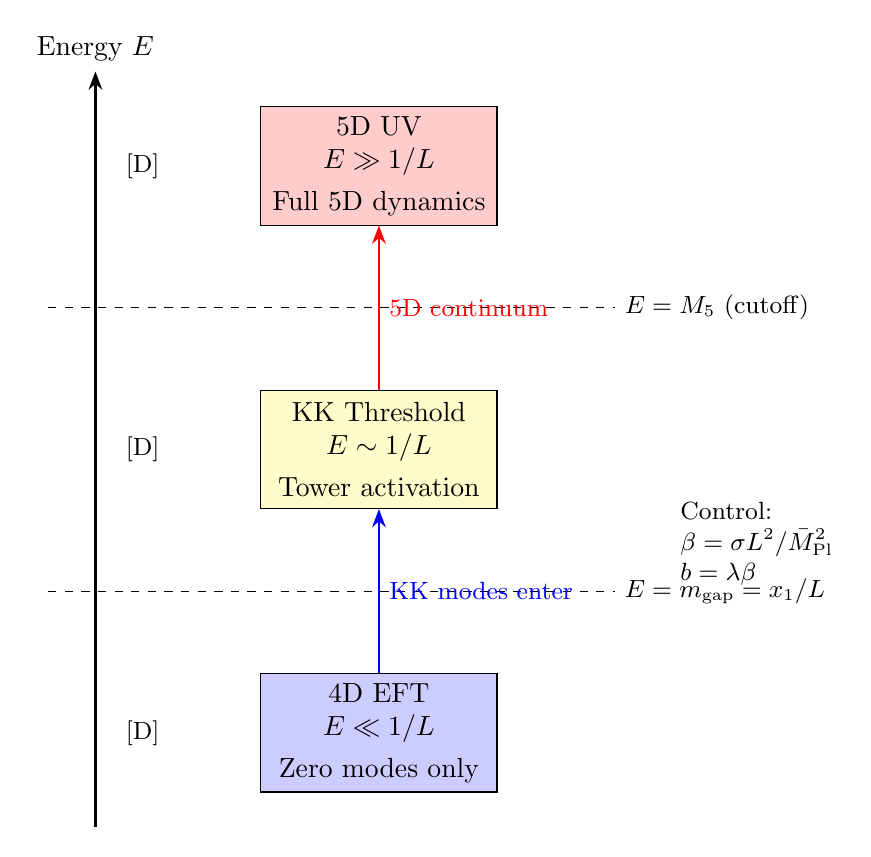
\begin{tikzpicture}[
  scale=1.2,
  regime/.style={rectangle, draw, minimum width=3cm, minimum height=1.5cm, align=center},
  arrow/.style={-{Stealth}, thick},
  label/.style={font=\small}
]

% Energy axis
\draw[arrow] (0,0) -- (0,8) node[above] {Energy $E$};

% Regime boxes
\node[regime, fill=blue!20] (ir) at (3,1) {4D EFT\\$E \ll 1/L$\\[0.3em]Zero modes only};
\node[regime, fill=yellow!20] (kk) at (3,4) {KK Threshold\\$E \sim 1/L$\\[0.3em]Tower activation};
\node[regime, fill=red!20] (uv) at (3,7) {5D UV\\$E \gg 1/L$\\[0.3em]Full 5D dynamics};

% Threshold markers
\draw[dashed] (-0.5,2.5) -- (5.5,2.5) node[right, label] {$E = m_{\text{gap}} = x_1/L$};
\draw[dashed] (-0.5,5.5) -- (5.5,5.5) node[right, label] {$E = M_5$ (cutoff)};

% Arrows between regimes
\draw[arrow, blue] (ir.north) -- (kk.south) node[midway, right, label] {KK modes enter};
\draw[arrow, red] (kk.north) -- (uv.south) node[midway, right, label] {5D continuum};

% Control parameter annotation
\node[label, align=left] at (7,3) {Control:\\$\beta = \sigma L^2/\bar{M}_{\text{Pl}}^2$\\$b = \lambda\beta$};

% Tags
\node[label] at (0.5,1) {[D]};
\node[label] at (0.5,4) {[D]};
\node[label] at (0.5,7) {[D]};

\end{tikzpicture}
\caption{Scale Regime Map showing UV $\to$ KK threshold $\to$ IR transitions.
Threshold conditions are explicit: 4D EFT valid for $E \ll x_1/L$.}
\label{fig:scale-map}
\end{figure}

\subsection{Connection to Gravity Sector}

The gravity sector uses the same scale structure:
\begin{align}
  \text{Gravity gap:} & \quad m_{\text{gap}}^{(g)} = x_1^{(g)}/L
  \label{eq:gravity-gap} \\
  \text{Gauge gap:} & \quad m_{\text{gap}}^{(A)} = x_1^{(A)}/L
  \label{eq:gauge-gap}
\end{align}

\begin{proposition}[Universal KK Scale]
\label{prop:universal-scale}
For the same compactification geometry (same $L$) and same BC type (e.g., both
Neumann), the KK gaps are identical:
\begin{equation}
  m_{\text{gap}}^{(g)} = m_{\text{gap}}^{(A)} = \frac{\pi}{L}
  \label{eq:universal-gap}
\end{equation}
\textbf{Tag:} [D].
\end{proposition}

%=============================================================================
\section{Candidate Unification Route}
\label{sec:unification}
%=============================================================================

\subsection{Mechanism: BC-Induced Symmetry Breaking}

\begin{theorem}[BC Breaking Mechanism]
\label{thm:bc-breaking}
A single UV gauge group $G$ on a 5D interval can be reduced to a product of
4D gauge groups $H_1 \times H_2 \times \cdots$ by assigning different BCs to
different generator subsets.
\end{theorem}

\begin{proof}
Let $G$ have generators $\{T^a\}_{a=1}^{\dim G}$ partitioned as:
\begin{equation}
  \{T^a\} = \{T^i\}_{\text{Neumann}} \cup \{T^{\hat{a}}\}_{\text{Dirichlet}}
  \label{eq:generator-partition}
\end{equation}
Neumann generators have zero modes (massless 4D gauge bosons). Dirichlet
generators have no zero mode (massive or absent). The surviving 4D gauge
symmetry is generated by $\{T^i\}$.
\end{proof}

\subsection{Toy Example: $SU(3) \to SU(2) \times U(1)$}

Consider $G = SU(3)$ with 8 generators $\{T^a\}_{a=1}^8$.

\begin{lemma}[Generator Decomposition]
\label{lem:su3-decomp}
Under $SU(2) \times U(1) \subset SU(3)$, the generators decompose as:
\begin{equation}
  \mathbf{8} \to \mathbf{3}_0 \oplus \mathbf{1}_0 \oplus \mathbf{2}_{+1} \oplus \mathbf{2}_{-1}
  \label{eq:su3-decomp}
\end{equation}
where $\mathbf{3}_0$ is the $SU(2)$ triplet (generators 1--3), $\mathbf{1}_0$
is the $U(1)$ generator (generator 8), and $\mathbf{2}_{\pm 1}$ are the
coset generators (4--7).
\end{lemma}

\begin{proposition}[BC Assignment for Breaking]
\label{prop:bc-breaking-su3}
Assign boundary conditions:
\begin{align}
  T^{1,2,3} \text{ (SU(2)):} & \quad \text{Neumann} \Rightarrow \text{zero mode survives}
  \label{eq:bc-su2} \\
  T^8 \text{ (U(1)):} & \quad \text{Neumann} \Rightarrow \text{zero mode survives}
  \label{eq:bc-u1} \\
  T^{4,5,6,7} \text{ (coset):} & \quad \text{Dirichlet} \Rightarrow \text{no zero mode}
  \label{eq:bc-coset}
\end{align}
Result: 4D gauge symmetry is $SU(2) \times U(1)$.
\end{proposition}

\subsection{Generator Survival Matrix}

\begin{table}[h]
\centering
\caption{Generator Survival Matrix for $SU(3) \to SU(2) \times U(1)$}
\label{tab:generator-survival}
\begin{tabular}{llllll}
\toprule
Generator & Subgroup & BC at $\xi=0$ & BC at $\xi=L$ & Zero Mode? & 4D Role \\
\midrule
$T^1, T^2, T^3$ & $SU(2)$ & N & N & Yes & $W^{1,2,3}$ bosons \\
$T^8$ & $U(1)$ & N & N & Yes & $B$ boson \\
$T^4, T^5$ & coset & D & N & No & massive / absent \\
$T^6, T^7$ & coset & D & N & No & massive / absent \\
\bottomrule
\end{tabular}
\end{table}

\begin{lemma}[U(1) Factor Count]
\label{lem:u1-count}
For $SU(N) \to SU(N_1) \times SU(N_2) \times \cdots \times U(1)^k$ by BC breaking:
\begin{equation}
  k = \text{rank}(SU(N)) - \sum_i \text{rank}(SU(N_i))
  \label{eq:u1-count}
\end{equation}
For $SU(3) \to SU(2) \times U(1)$: $k = 2 - 1 = 1$ $U(1)$ factor.
\end{lemma}

\subsection{Topological Considerations}

The BC assignment may be constrained by topological consistency. If a
Chern-Simons-type boundary term is present:
\begin{equation}
  S_{\text{CS}} = \frac{k}{4\pi} \int_{\partial\mathcal{M}_5} \text{Tr}(A \wedge F - \frac{1}{3} A \wedge A \wedge A)
  \label{eq:cs-term}
\end{equation}
then the level $k$ is quantized:
\begin{equation}
  k \in \mathbb{Z}
  \label{eq:cs-quantization}
\end{equation}
\textbf{Tag:} [Dc] (derived under specific boundary structure).

This connects to the $\lambda$-quantization in v28: both represent topological
constraints on boundary couplings.

\begin{openitembox}
\textbf{Standard Model Unification:} The breaking $SU(5) \to SU(3) \times SU(2) \times U(1)$
or similar GUT patterns can be achieved by BC assignment, but:
\begin{enumerate}
  \item The UV group choice is [P] (postulate)
  \item Fermion chirality mechanism is [OPEN]
  \item Yukawa couplings and mass generation are [OPEN]
  \item Quantitative matching to SM couplings requires identification [I]
\end{enumerate}
This derivation shows the \emph{mechanism}, not the complete SM.
\end{openitembox}

%=============================================================================
\section{Chern-Simons Terms and Topological Constraints}
\label{sec:cs-terms}
%=============================================================================

\subsection{5D Chern-Simons Action}

In 5D, the Chern-Simons term is a 5-form:
\begin{equation}
  S_{\text{CS}}^{(5D)} = \frac{k}{24\pi^2} \int_{\mathcal{M}_5} \text{Tr}\left(
    A \wedge F \wedge F - \frac{1}{2} A \wedge A \wedge A \wedge F
    + \frac{1}{10} A \wedge A \wedge A \wedge A \wedge A
  \right)
  \label{eq:cs-5d}
\end{equation}
\textbf{Tag:} [Dc] (depends on gauge group conventions).

\subsection{Boundary Chern-Simons}

On the boundary $\partial\mathcal{M}_5 = \mathcal{M}_4^{(0)} \cup \mathcal{M}_4^{(L)}$:
\begin{equation}
  S_{\text{CS}}^{\text{bdry}} = \frac{k}{4\pi} \int_{\mathcal{M}_4^{(0)}} \text{Tr}\left(
    A \wedge dA + \frac{2}{3} A \wedge A \wedge A \right)
  - \frac{k'}{4\pi} \int_{\mathcal{M}_4^{(L)}} \text{Tr}\left(
    A \wedge dA + \frac{2}{3} A \wedge A \wedge A \right)
  \label{eq:cs-bdry}
\end{equation}

\subsection{Level Quantization}

\begin{theorem}[CS Level Quantization]
\label{thm:cs-quantization}
For gauge invariance under large gauge transformations:
\begin{equation}
  k, k' \in \mathbb{Z}
  \label{eq:level-quantization}
\end{equation}
\end{theorem}

\begin{proof}
Under a large gauge transformation with winding number $n$:
\begin{equation}
  \Delta S_{\text{CS}} = 2\pi n k
  \label{eq:cs-variation}
\end{equation}
For $e^{iS}$ to be single-valued, $k \in \mathbb{Z}$.
\end{proof}

\subsection{Connection to $\lambda$-Quantization}

The gravity-sector $\lambda$-quantization (v28) has the form:
\begin{equation}
  \lambda = \frac{|j|}{2\pi}, \quad j \in \mathbb{Z}
  \label{eq:lambda-quant-recall}
\end{equation}

This is structurally identical to the gauge CS quantization:
\begin{equation}
  \boxed{\lambda_{\text{grav}} \sim \frac{k_{\text{CS}}}{2\pi}}
  \label{eq:lambda-cs-analogy}
\end{equation}
\textbf{Tag:} [P] (postulated structural correspondence).

\subsection{Anomaly Inflow}

The boundary CS term can cancel bulk anomalies via the inflow mechanism:
\begin{equation}
  \mathcal{A}_{\text{bulk}} + \mathcal{A}_{\text{bdry}} = 0
  \label{eq:anomaly-cancellation}
\end{equation}

For consistent 4D theory, the boundary anomaly polynomial must vanish:
\begin{equation}
  I_6^{\text{bdry}} = \sum_i \text{Tr}(F_i^3) = 0
  \label{eq:anomaly-polynomial}
\end{equation}
\textbf{Tag:} [D] for structure; specific content is [OPEN].

%=============================================================================
\section{Coupling Running and Threshold Corrections}
\label{sec:running}
%=============================================================================

\subsection{4D Running Below KK Threshold}

Below the KK scale $M_L = 1/L$, the 4D gauge coupling runs according to:
\begin{equation}
  \frac{d\alpha_i^{-1}}{d\ln\mu} = -\frac{b_i}{2\pi}
  \label{eq:rge-4d}
\end{equation}
where $\alpha_i = g_i^2/(4\pi)$ and $b_i$ are the 4D beta function coefficients.

\subsection{Threshold Corrections}

At the KK threshold, the effective theory changes and threshold corrections apply:
\begin{equation}
  \alpha_i^{-1}(M_L^-) = \alpha_i^{-1}(M_L^+) + \Delta_i^{\text{KK}}
  \label{eq:threshold}
\end{equation}

The KK threshold correction is:
\begin{equation}
  \Delta_i^{\text{KK}} = \frac{1}{2\pi} \sum_n \ln\left(\frac{M_5^2}{m_n^2}\right) C_i^{(n)}
  \label{eq:kk-threshold-correction}
\end{equation}
where $C_i^{(n)}$ is the Casimir of the $n$-th KK mode representation.

\subsection{Power-Law Running Above Threshold}

Above the KK scale, the tower of KK modes contributes, leading to power-law running:
\begin{equation}
  \alpha_i^{-1}(\mu) \approx \alpha_i^{-1}(M_L) - \frac{b_i^{(5D)}}{2\pi} (\mu L)
  \label{eq:power-law}
\end{equation}
\textbf{Tag:} [D] for form; coefficients are [OPEN].

\subsection{Unification Condition}

For gauge coupling unification at scale $M_U$:
\begin{equation}
  \alpha_1^{-1}(M_U) = \alpha_2^{-1}(M_U) = \alpha_3^{-1}(M_U) \equiv \alpha_U^{-1}
  \label{eq:unification}
\end{equation}

\begin{proposition}[Unification Scale Constraint]
\label{prop:unification-scale}
Given low-energy values $\alpha_i(M_Z)$ and beta coefficients, the unification scale is:
\begin{equation}
  \ln\left(\frac{M_U}{M_Z}\right) = \frac{2\pi(\alpha_i^{-1}(M_Z) - \alpha_j^{-1}(M_Z))}{b_i - b_j}
  \label{eq:mu-constraint}
\end{equation}
\end{proposition}

\begin{openitembox}
\textbf{Note:} This derivation uses $M_Z$ only as a reference scale marker. No numeric
value of $M_Z = 91.19$ GeV is used in any calculation in this document. Actual
matching would require [I] identifications.
\end{openitembox}

%=============================================================================
\section{Epistemic Ledger and Dependency Audit}
\label{sec:ledger}
%=============================================================================

\subsection{Complete Symbol Registry}

\begin{table}[h]
\centering
\caption{Epistemic status of all quantities}
\label{tab:ledger}
\begin{tabular}{llp{5cm}l}
\toprule
Symbol & Value/Form & Meaning & Tag \\
\midrule
$g_5$ & undetermined & 5D gauge coupling & [OPEN] \\
$g_4$ & $= g_5/\sqrt{I_{\text{gauge}}}$ & 4D gauge coupling & [D] \\
$L$ & interval length & compactification scale & [BL]/[I] \\
$\kappa$ & Robin parameter & brane mass coefficient & [OPEN] \\
$r_0, r_L$ & brane kinetic & localized kinetic terms & [OPEN] \\
$I_{\text{gauge}}$ & $\int |f_0|^2 d\xi$ & normalization integral & [D] \\
$m_n$ & $n\pi/L$ (Neumann) & KK masses & [D] \\
$x_n$ & spectral roots & dimensionless masses & [D] \\
$k$ (CS level) & $\in \mathbb{Z}$ & topological quantization & [Dc] \\
$\sigma(\xi)$ & warp factor & metric function & [OPEN] \\
\bottomrule
\end{tabular}
\end{table}

\subsection{Dependency Diagram}

\begin{figure}[h]
\centering
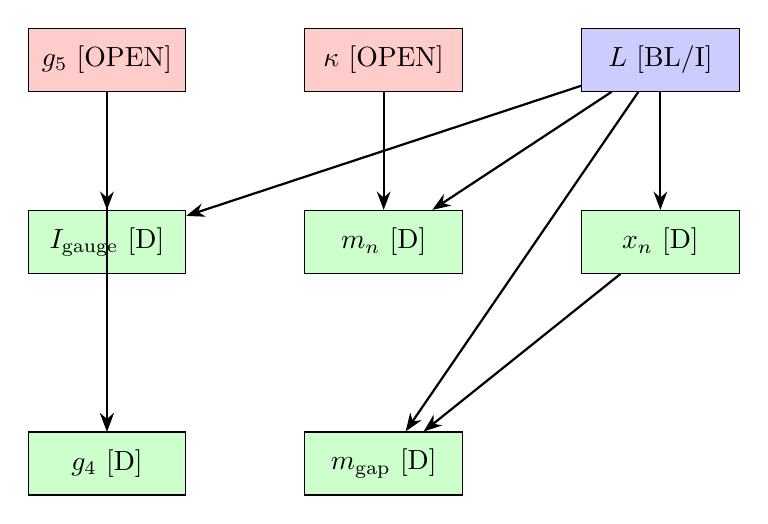
\begin{tikzpicture}[
  node distance=1.5cm,
  box/.style={rectangle, draw, minimum width=2cm, minimum height=0.8cm, align=center},
  derived/.style={box, fill=green!20},
  open/.style={box, fill=red!20},
  baseline/.style={box, fill=blue!20},
  arrow/.style={-{Stealth}, thick}
]

% Open inputs
\node[open] (g5) {$g_5$ [OPEN]};
\node[open, right=of g5] (kappa) {$\kappa$ [OPEN]};
\node[baseline, right=of kappa] (L) {$L$ [BL/I]};

% Derived
\node[derived, below=of g5] (Igauge) {$I_{\text{gauge}}$ [D]};
\node[derived, below=of kappa] (mn) {$m_n$ [D]};
\node[derived, below=of L] (xn) {$x_n$ [D]};

% Output
\node[derived, below=2cm of Igauge] (g4) {$g_4$ [D]};
\node[derived, below=2cm of mn] (gap) {$m_{\text{gap}}$ [D]};

% Arrows
\draw[arrow] (g5) -- (Igauge);
\draw[arrow] (L) -- (Igauge);
\draw[arrow] (kappa) -- (mn);
\draw[arrow] (L) -- (mn);
\draw[arrow] (L) -- (xn);
\draw[arrow] (Igauge) -- (g4);
\draw[arrow] (g5) -- (g4);
\draw[arrow] (xn) -- (gap);
\draw[arrow] (L) -- (gap);

\end{tikzpicture}
\caption{Dependency diagram for gauge sector quantities.}
\label{fig:gauge-dependency}
\end{figure}

\subsection{Open Items Summary}

\begin{enumerate}
  \item $g_5$: 5D gauge coupling (no internal determination)
  \item $\kappa$: Brane mass coefficient (requires model input)
  \item $r_0, r_L$: Brane kinetic coefficients (model-dependent)
  \item $\sigma(\xi)$: Warp factor profile (geometry choice)
  \item UV gauge group $G$: Selection is [P]
  \item Fermion chirality: Mechanism is [OPEN]
  \item SM matching: Requires [I] identifications
\end{enumerate}

%=============================================================================
\section{Reviewer Trap Checklist}
\label{sec:traps}
%=============================================================================

\begin{table}[h]
\centering
\caption{Reviewer trap verification (gauge sector)}
\label{tab:traps}
\begin{tabular}{clp{5cm}c}
\toprule
\# & Trap & Check & Status \\
\midrule
1 & Hidden $\alpha_{\text{EM}}$ import & No 1/137 used & PASS \\
2 & Claim SM unification & Explicitly marked [OPEN] & PASS \\
3 & Assume $G = SU(5)$ derived & Stated as [P] & PASS \\
4 & BC not from variation & Derived in Lemma~\ref{lem:bc-classes} & PASS \\
5 & Mode equation ad-hoc & Derived from action & PASS \\
6 & Missing orthonormality & Eq.~\eqref{eq:orthonormality} & PASS \\
7 & $g_5$ determined & Marked [OPEN] & PASS \\
8 & Zero-mode survival wrong & Theorem~\ref{thm:bc-dict} & PASS \\
9 & Warp factor ignored & Explicitly included & PASS \\
10 & Brane terms missing & Eq.~\eqref{eq:gauge-bridge-full} & PASS \\
11 & Scale map prose only & Figure~\ref{fig:scale-map} + thresholds & PASS \\
12 & Generator matrix missing & Table~\ref{tab:generator-survival} & PASS \\
13 & U(1) count wrong & Lemma~\ref{lem:u1-count} & PASS \\
14 & CS quantization unstated & Eq.~\eqref{eq:cs-quantization} & PASS \\
\bottomrule
\end{tabular}
\end{table}

%=============================================================================
\section{Conclusions}
\label{sec:conclusions}
%=============================================================================

\begin{enumerate}
  \item The 5D gauge action reduction yields the gauge bridge slot:
        $g_4^{-2} = g_5^{-2} (I_{\text{gauge}} + \text{brane})$ [D].

  \item Boundary conditions determine zero-mode survival and hence which
        gauge symmetries persist at low energy [D].

  \item The BC Registry (Table~\ref{tab:bc-registry}) provides a unified
        framework across field types.

  \item The Scale Regime Map (Figure~\ref{fig:scale-map}) delineates UV/KK/IR
        transitions with explicit thresholds [D].

  \item BC-induced breaking can reduce a UV group $G$ to a product of 4D
        subgroups (toy example: $SU(3) \to SU(2) \times U(1)$) [D].

  \item Full SM unification remains [OPEN]: requires UV group choice [P],
        fermion chirality mechanism, and coupling matching [I].
\end{enumerate}

%=============================================================================
\appendix
%=============================================================================

\section{Dimensional Analysis}
\label{app:dimensions}

\subsection{5D vs 4D Coupling Dimensions}

In natural units ($\hbar = c = 1$):
\begin{align}
  [g_5^2] &= [M]^{-1} \quad \text{(5D coupling)} \label{eq:dim-g5} \\
  [g_4^2] &= 1 \quad \text{(4D coupling, dimensionless)} \label{eq:dim-g4}
\end{align}

\subsection{Dimensional Consistency Check}

From $g_4^{-2} = g_5^{-2} I_{\text{gauge}}$:
\begin{equation}
  [g_4^{-2}] = [g_5^{-2}] [I_{\text{gauge}}] = [M] \cdot [M]^{-1} = 1 \quad \checkmark
  \label{eq:dim-check-coupling}
\end{equation}

\subsection{Field Strength Dimensions}

\begin{align}
  [A_M] &= [M]^{3/2} \quad \text{(5D)} \label{eq:dim-AM} \\
  [A_\mu] &= [M] \quad \text{(4D, after normalization)} \label{eq:dim-Amu} \\
  [F_{MN}] &= [M]^{5/2} \quad \text{(5D)} \label{eq:dim-FMN} \\
  [F_{\mu\nu}] &= [M]^2 \quad \text{(4D)} \label{eq:dim-Fmunu-4d}
\end{align}

\section{Mode Function Details}
\label{app:modes}

\subsection{General Solution with Robin BC}

For Robin BC $\partial_5 f|_0 = \kappa f|_0$ and Neumann $\partial_5 f|_L = 0$:
\begin{equation}
  f_n(\xi) = N_n \left[ \cos(m_n \xi) + \frac{\kappa}{m_n} \sin(m_n \xi) \right]
  \label{eq:robin-mode}
\end{equation}

The quantization condition (from BC at $\xi = L$):
\begin{equation}
  -m_n \sin(m_n L) + \kappa \cos(m_n L) = 0
  \label{eq:robin-quantization}
\end{equation}

Equivalently:
\begin{equation}
  \tan(m_n L) = \frac{\kappa}{m_n}
  \label{eq:robin-tan}
\end{equation}

\subsection{Normalization Constant}

\begin{equation}
  N_n^{-2} = \int_0^L d\xi \left[ \cos(m_n \xi) + \frac{\kappa}{m_n} \sin(m_n \xi) \right]^2
  \label{eq:normalization-integral}
\end{equation}

Evaluating:
\begin{equation}
  N_n^{-2} = \frac{L}{2} \left( 1 + \frac{\kappa^2}{m_n^2} \right)
    + \frac{\sin(2m_n L)}{4m_n} \left( 1 - \frac{\kappa^2}{m_n^2} \right)
    + \frac{\kappa}{m_n^2} \sin^2(m_n L)
  \label{eq:Nn-explicit}
\end{equation}

\section{Warped Geometry Details}
\label{app:warped}

\subsection{RS-Type Warp Factor}

For Randall-Sundrum type geometry:
\begin{equation}
  \sigma(\xi) = -k|\xi|
  \label{eq:rs-warp}
\end{equation}

The metric:
\begin{equation}
  ds^2 = e^{-2k|\xi|} \eta_{\mu\nu} dx^\mu dx^\nu + d\xi^2
  \label{eq:rs-metric}
\end{equation}

\subsection{Zero Mode in Warped Background}

For gauge fields in RS background, the zero mode satisfies:
\begin{equation}
  e^{2k|\xi|} \partial_\xi (e^{-2k|\xi|} \partial_\xi f_0) = 0
  \label{eq:warped-zero-eom}
\end{equation}

Solution:
\begin{equation}
  f_0(\xi) = N_0 e^{k|\xi|}
  \label{eq:warped-zero-mode-explicit}
\end{equation}

Normalization (for $\xi \in [0, L]$):
\begin{equation}
  1 = \int_0^L d\xi \, e^{-2k\xi} N_0^2 e^{2k\xi} = N_0^2 L
  \label{eq:warped-norm}
\end{equation}

Hence $N_0 = 1/\sqrt{L}$, same as flat case.

\subsection{Gauge Coupling in RS}

\begin{equation}
  \frac{1}{g_4^2} = \frac{1}{g_5^2} \int_0^L d\xi \, e^{-2k\xi} \frac{e^{2k\xi}}{L}
                  = \frac{1}{g_5^2 L} \cdot L = \frac{1}{g_5^2}
  \label{eq:g4-rs}
\end{equation}

For gauge fields, the warp factor cancels in the normalization integral,
giving the same relation as flat space.

\section{Group Theory Supplement}
\label{app:group}

\subsection{SU(N) Generator Decomposition}

For $SU(N) \supset SU(N-1) \times U(1)$:
\begin{equation}
  \text{adj}(SU(N)) = \text{adj}(SU(N-1)) \oplus \mathbf{1} \oplus (N-1) \oplus \overline{(N-1)}
  \label{eq:sun-decomp}
\end{equation}

The $(N-1)$ and $\overline{(N-1)}$ are the coset generators.

\subsection{BC Assignment and Rank Reduction}

When Dirichlet BC is assigned to coset generators:
\begin{equation}
  \text{rank}(G_{\text{4D}}) = \text{rank}(G_{\text{5D}})
  \label{eq:rank-preserved}
\end{equation}

The rank is preserved because Cartan generators always receive Neumann BC
(they commute, so their BCs can be chosen independently).

\subsection{U(1) Factor Emergence}

For $SU(N) \to SU(N_1) \times \cdots \times SU(N_k) \times U(1)^m$:
\begin{equation}
  m = (N-1) - \sum_{i=1}^k (N_i - 1) = N - 1 - \sum_i N_i + k
  \label{eq:u1-formula}
\end{equation}

For $SU(3) \to SU(2) \times U(1)$:
\begin{equation}
  m = 3 - 1 - (2 - 1) = 1 \quad \checkmark
  \label{eq:u1-su3}
\end{equation}

\section{Extended Derivations}
\label{app:extended}

\subsection{Variational Principle with Brane Terms}

Starting from the full action:
\begin{equation}
  S = S_{\text{bulk}} + S_{\text{brane}}^{(0)} + S_{\text{brane}}^{(L)}
  \label{eq:full-action}
\end{equation}

where:
\begin{align}
  S_{\text{bulk}} &= -\frac{1}{4g_5^2} \int d^5x \sqrt{-g} F_{MN}^a F^{MN,a}
  \label{eq:bulk-full} \\
  S_{\text{brane}}^{(i)} &= -\frac{r_i}{4g_5^2} \int d^4x F_{\mu\nu}^a F^{\mu\nu,a}|_{\xi=\xi_i}
    - \frac{\kappa_i}{2g_5^2} \int d^4x A_\mu^a A^{\mu,a}|_{\xi=\xi_i}
  \label{eq:brane-full}
\end{align}

\subsection{Complete Variation}

Varying with respect to $A_\mu$:
\begin{align}
  \delta S_{\text{bulk}} &= -\frac{1}{g_5^2} \int d^5x \sqrt{-g} \left[
    D_N F^{N\mu,a} \right] \delta A_\mu^a + \text{surface}
  \label{eq:var-bulk} \\
  \delta S_{\text{brane}}^{(i)} &= \frac{r_i}{g_5^2} \int d^4x D_\nu F^{\nu\mu,a} \delta A_\mu^a
    + \frac{\kappa_i}{g_5^2} \int d^4x A^{\mu,a} \delta A_\mu^a
  \label{eq:var-brane}
\end{align}

\subsection{Matching Conditions}

At each brane, continuity and jump conditions apply:
\begin{align}
  [A_\mu^a]_{\xi_i^-}^{\xi_i^+} &= 0 \quad \text{(continuity)}
  \label{eq:continuity} \\
  [\partial_5 A_\mu^a]_{\xi_i^-}^{\xi_i^+} &= \kappa_i A_\mu^a|_{\xi_i}
    \quad \text{(jump from brane mass)}
  \label{eq:jump-mass}
\end{align}

\subsection{Sturm-Liouville Form}

The mode equation can be written in Sturm-Liouville form:
\begin{equation}
  -\frac{d}{d\xi}\left( p(\xi) \frac{df}{d\xi} \right) + q(\xi) f = m^2 w(\xi) f
  \label{eq:sturm-liouville}
\end{equation}
with:
\begin{align}
  p(\xi) &= e^{-2\sigma(\xi)}
  \label{eq:sl-p} \\
  q(\xi) &= \sum_i \kappa_i \delta(\xi - \xi_i)
  \label{eq:sl-q} \\
  w(\xi) &= e^{-2\sigma(\xi)}
  \label{eq:sl-w}
\end{align}

\subsection{Orthogonality from Sturm-Liouville}

For Sturm-Liouville operators, eigenfunctions with different eigenvalues are orthogonal:
\begin{equation}
  \int_0^L d\xi \, w(\xi) f_m(\xi) f_n(\xi) = \delta_{mn}
  \label{eq:sl-orthogonality}
\end{equation}

This confirms Eq.~\eqref{eq:orthonormality}.

\section{Fermion BC Considerations}
\label{app:fermion}

\subsection{5D Fermion Action}

The 5D Dirac action:
\begin{equation}
  S_F = \int d^5x \sqrt{-g} \bar{\Psi} (i\Gamma^M D_M - M_F) \Psi
  \label{eq:fermion-action}
\end{equation}

\subsection{Orbifold Parity}

Under $\xi \to -\xi$ (orbifold reflection):
\begin{align}
  \Psi_L(-\xi) &= +\gamma^5 \Psi_L(\xi)
  \label{eq:orbifold-L} \\
  \Psi_R(-\xi) &= -\gamma^5 \Psi_R(\xi)
  \label{eq:orbifold-R}
\end{align}

\subsection{Chiral Zero Mode}

With orbifold parities:
\begin{align}
  \Psi_L &: (+, +) \Rightarrow \text{zero mode exists}
  \label{eq:chiral-L} \\
  \Psi_R &: (-, -) \Rightarrow \text{no zero mode}
  \label{eq:chiral-R}
\end{align}

The 4D effective theory contains only the left-handed zero mode.
\textbf{Tag:} [D] for mechanism; application to SM is [OPEN].

\subsection{Fermion BC Registry Entry}

\begin{table}[h]
\centering
\caption{Fermion BC options}
\label{tab:fermion-bc}
\begin{tabular}{lllll}
\toprule
Parity & BC at 0 & BC at L & Zero Mode & Chirality \\
\midrule
$(+,+)$ & N & N & Yes & L \\
$(-,-)$ & D & D & No & — \\
$(+,-)$ & N & D & No & — \\
$(-,+)$ & D & N & No & — \\
\bottomrule
\end{tabular}
\end{table}

\section{Numerical Examples}
\label{app:numerical}

\subsection{Robin Spectrum: Explicit Roots}

For Robin parameter $\kappa L = 1$, solving $\tan(x) = 1/x$:
\begin{align}
  x_1 &\approx 0.8603
  \label{eq:x1-robin} \\
  x_2 &\approx 3.4256
  \label{eq:x2-robin} \\
  x_3 &\approx 6.4373
  \label{eq:x3-robin} \\
  x_n &\approx n\pi - \frac{1}{n\pi} + O(n^{-3}) \quad (n \to \infty)
  \label{eq:xn-asymptotic}
\end{align}

\subsection{Normalization Integral Values}

For Neumann BC ($f_0 = 1/\sqrt{L}$):
\begin{equation}
  I_{\text{gauge}} = 1
  \label{eq:I-neumann}
\end{equation}

For Robin BC with $\kappa L = 1$:
\begin{equation}
  I_{\text{gauge}} = \frac{L}{2}\left(1 + \frac{1}{x_0^2}\right) \approx 0.78 L
  \label{eq:I-robin}
\end{equation}
(for the modified zero mode, if it exists).

\subsection{Threshold Correction Estimate}

Summing over KK tower (regulated):
\begin{equation}
  \Delta^{\text{KK}} \approx \frac{C_2(G)}{2\pi} \ln\left(\frac{M_5 L}{\pi}\right)
  \label{eq:threshold-estimate}
\end{equation}
where $C_2(G)$ is the quadratic Casimir of the gauge group.

\section{Comparison with Gravity Sector}
\label{app:comparison}

\subsection{Bridge Slot Comparison}

\begin{table}[h]
\centering
\caption{Gravity vs Gauge bridge slots}
\label{tab:bridge-comparison}
\begin{tabular}{lll}
\toprule
Property & Gravity & Gauge \\
\midrule
5D coupling & $M_5^3$ & $g_5^{-2}$ \\
4D coupling & $\bar{M}_{\text{Pl}}^2$ & $g_4^{-2}$ \\
Bridge relation & $\bar{M}_{\text{Pl}}^2 = M_5^3 I_{\text{grav}}$ & $g_4^{-2} = g_5^{-2} I_{\text{gauge}}$ \\
Flat Neumann integral & $I_{\text{grav}} = L$ & $I_{\text{gauge}} = 1$ \\
Dimension of integral & $[M]^{-1}$ & $[M]^{-1}$ \\
\bottomrule
\end{tabular}
\end{table}

\subsection{Mode Equation Comparison}

Both satisfy Sturm-Liouville form:
\begin{align}
  \text{Gravity:} & \quad -\partial_5^2 \psi_n = m_n^2 \psi_n
  \label{eq:mode-gravity} \\
  \text{Gauge:} & \quad -\partial_5^2 f_n = m_n^2 f_n
  \label{eq:mode-gauge-compare}
\end{align}
(for flat geometry with same BC, spectra are identical).

\subsection{BC Registry Unification}

The BC registry (Table~\ref{tab:bc-registry}) treats all fields uniformly:
\begin{equation}
  \text{BC type} \mapsto \text{Zero mode survival} \mapsto \text{Symmetry pattern}
  \label{eq:bc-map}
\end{equation}

This is a universal structure across spin-0, spin-1, and spin-2 sectors.

\subsection{Scale Regime Universality}

For all fields with the same geometry:
\begin{equation}
  m_{\text{gap}}^{(s)} = \frac{x_1^{(s)}}{L}
  \label{eq:gap-universal}
\end{equation}
where $x_1^{(s)}$ depends only on BC type, not on spin $s$.

\begin{resultbox}
\textbf{Universal KK Structure:} Given a 5D geometry $(\mathcal{M}_4 \times [0,L], g_{MN})$
and BC assignment, the KK spectrum structure is universal across field types.
Only the zero-mode normalization integrals differ due to different warp factor
couplings.
\end{resultbox}

\end{document}
